%% Auto-generated by fig_qualitative.py -- do not edit by hand.
\documentclass[border=0pt]{standalone}
\usepackage{iftex}
\ifPDFTeX
  \usepackage[T1]{fontenc}\usepackage{times}
\else
  \usepackage{fontspec}\setmainfont{texgyretermes}[Extension=.otf,UprightFont=*-regular,BoldFont=*-bold,ItalicFont=*-italic,BoldItalicFont=*-bolditalic]
\fi
\usepackage{graphicx}
\usepackage{tikz}
% Shared method colors for all figures/diagrams (same hexes as figures/src/figstyle.py).
% Validated colorblind-safe on white (all-pairs CVD dE >= 9.4, contrast >= 3.4:1); always pair with a
% second cue (marker shape, label) so identity never relies on hue alone.
\definecolor{cOurs}{HTML}{256ABF}      % Ours (KalSea + predictor-corrector gap smoothing)
\definecolor{cKalSea}{HTML}{199E70}    % KalSea (Kalman forecasting, no smoothing)
\definecolor{cSeaCache}{HTML}{D95926}  % SeaCache (SEA gate + residual reuse)
\definecolor{cReference}{HTML}{0B0B0B} % 50-step reference
\definecolor{cInk}{HTML}{0B0B0B}
\definecolor{cInkTwo}{HTML}{52514E}
\definecolor{cMuted}{HTML}{898781}
\definecolor{cGrid}{HTML}{E1E0D9}

\newcommand{\hdr}{\fontsize{7.5}{8.5}\selectfont}
\newcommand{\sub}{\fontsize{7}{8}\selectfont\color{cInkTwo}}
\newcommand{\prm}{\fontsize{7}{8.1}\selectfont\itshape\color{cInk}}
\newcommand{\num}{\fontsize{7}{8}\selectfont\color{cInk}}
\begin{document}
\begin{tikzpicture}[x=1bp,y=1bp,line join=round]
\path[use as bounding box] (0,0) rectangle (495.00,-490.95);
\node[anchor=south,inner sep=0] at (49.25,-21.80) {\hdr Reference};
\node[anchor=south,inner sep=0] at (49.25,-11.40) {\sub 50 NFE};
\draw[cMuted,line width=0.4bp] (11.00,-12.40) -- (87.50,-12.40);
\node[anchor=south,inner sep=0] at (169.25,-11.40) {\sub 20--21 NFE, identical computed steps};
\draw[cMuted,line width=0.4bp] (91.00,-12.40) -- (247.50,-12.40);
\node[anchor=south,inner sep=0] (h01) at (132.25,-21.80) {\hdr SeaCache};
\path (h01.west) ++(-4.0,1.9) coordinate (mk);
\begin{scope}[shift={(mk)}]\fill[cSeaCache] (-2.10,-2.10) rectangle (2.10,2.10);\end{scope}
\node[anchor=south,inner sep=0] (h02) at (212.25,-21.80) {\hdr KalSea};
\path (h02.west) ++(-4.0,1.9) coordinate (mk);
\begin{scope}[shift={(mk)}]\fill[cOurs] (0.00,-0.25) circle (2.21);\end{scope}
\node[anchor=south,inner sep=0] at (295.75,-21.80) {\hdr Reference};
\node[anchor=south,inner sep=0] at (295.75,-11.40) {\sub 50 NFE};
\draw[cMuted,line width=0.4bp] (257.50,-12.40) -- (334.00,-12.40);
\node[anchor=south,inner sep=0] at (415.75,-11.40) {\sub 20--21 NFE, identical computed steps};
\draw[cMuted,line width=0.4bp] (337.50,-12.40) -- (494.00,-12.40);
\node[anchor=south,inner sep=0] (h11) at (378.75,-21.80) {\hdr SeaCache};
\path (h11.west) ++(-4.0,1.9) coordinate (mk);
\begin{scope}[shift={(mk)}]\fill[cSeaCache] (-2.10,-2.10) rectangle (2.10,2.10);\end{scope}
\node[anchor=south,inner sep=0] (h12) at (458.75,-21.80) {\hdr KalSea};
\path (h12.west) ++(-4.0,1.9) coordinate (mk);
\begin{scope}[shift={(mk)}]\fill[cOurs] (0.00,-0.25) circle (2.21);\end{scope}
\node[anchor=south west,inner sep=0,text width=238.50bp,align=flush left,font=\prm] at (10.00,-40.50) {``New York Skyline with `Diffusion' written with fireworks on the sky.''};
\node[anchor=north west,inner sep=0] at (10.00,-42.50) {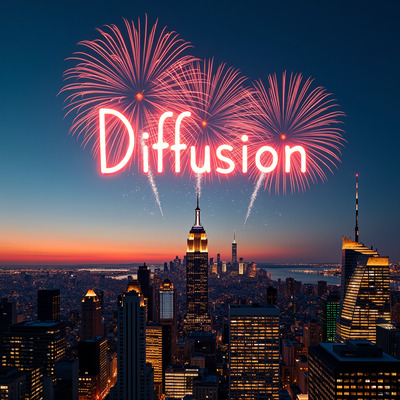
\includegraphics[width=78.500bp,height=78.500bp]{qual_tiles/nfe21_supp/194_reference_full.jpg}};
\draw[black,line width=1.3bp] (41.89,-60.29) rectangle (61.52,-70.10);
\draw[white,line width=0.6bp] (41.89,-60.29) rectangle (61.52,-70.10);
\node[anchor=north west,inner sep=0] at (10.00,-122.50) {
\includegraphics[width=78.500bp,height=39.250bp]{qual_tiles/nfe21_supp/194_reference_crop.jpg}};
\node[anchor=north,inner sep=0] at (49.25,-163.55) {\num\color{cInkTwo}PSNR (dB)};
\node[anchor=north west,inner sep=0] at (90.00,-42.50) {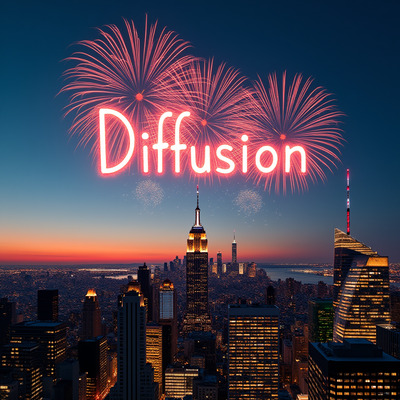
\includegraphics[width=78.500bp,height=78.500bp]{qual_tiles/nfe21_supp/194_seacache_full.jpg}};
\draw[black,line width=1.3bp] (121.89,-60.29) rectangle (141.52,-70.10);
\draw[white,line width=0.6bp] (121.89,-60.29) rectangle (141.52,-70.10);
\node[anchor=north west,inner sep=0] at (90.00,-122.50) {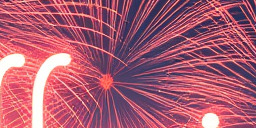
\includegraphics[width=78.500bp,height=39.250bp]{qual_tiles/nfe21_supp/194_seacache_crop.jpg}};
\node[anchor=north,inner sep=0] at (129.25,-163.55) {\num 22.82};
\node[anchor=north west,inner sep=0] at (170.00,-42.50) {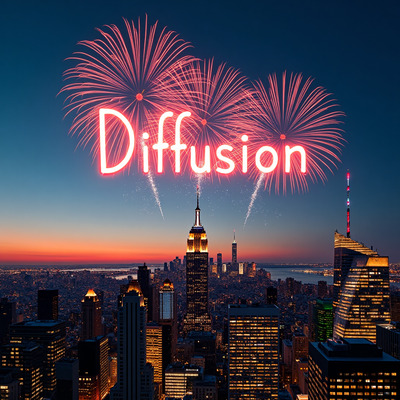
\includegraphics[width=78.500bp,height=78.500bp]{qual_tiles/nfe21_supp/194_ours_full.jpg}};
\draw[black,line width=1.3bp] (201.89,-60.29) rectangle (221.52,-70.10);
\draw[white,line width=0.6bp] (201.89,-60.29) rectangle (221.52,-70.10);
\node[anchor=north west,inner sep=0] at (170.00,-122.50) {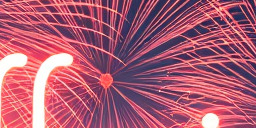
\includegraphics[width=78.500bp,height=39.250bp]{qual_tiles/nfe21_supp/194_ours_crop.jpg}};
\node[anchor=north,inner sep=0] at (209.25,-163.55) {\num \textbf{23.87}};
\node[rotate=90,anchor=south,inner sep=0] at (6.80,-102.12) {\sub Lower-quartile gain};
\node[anchor=south west,inner sep=0,text width=238.50bp,align=flush left,font=\prm] at (256.50,-40.50) {``Rainbow coloured penguin.''};
\node[anchor=north west,inner sep=0] at (256.50,-42.50) {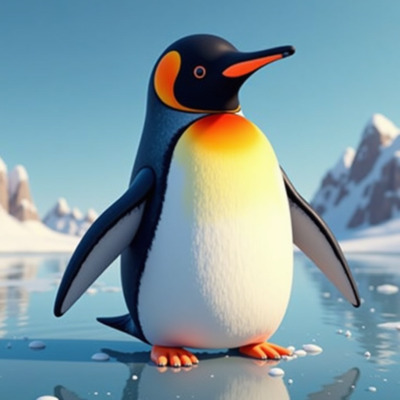
\includegraphics[width=78.500bp,height=78.500bp]{qual_tiles/nfe21_supp/033_reference_full.jpg}};
\draw[black,line width=1.3bp] (294.52,-48.63) rectangle (314.15,-58.45);
\draw[white,line width=0.6bp] (294.52,-48.63) rectangle (314.15,-58.45);
\node[anchor=north west,inner sep=0] at (256.50,-122.50) {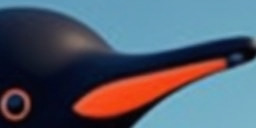
\includegraphics[width=78.500bp,height=39.250bp]{qual_tiles/nfe21_supp/033_reference_crop.jpg}};
\node[anchor=north,inner sep=0] at (295.75,-163.55) {\num\color{cInkTwo}PSNR (dB)};
\node[anchor=north west,inner sep=0] at (336.50,-42.50) {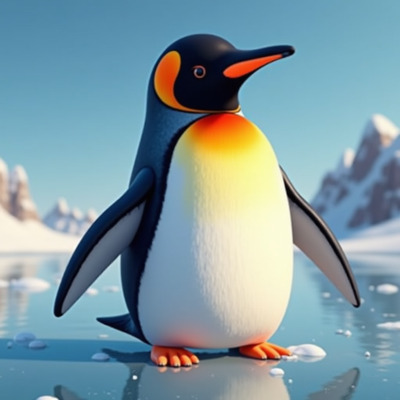
\includegraphics[width=78.500bp,height=78.500bp]{qual_tiles/nfe21_supp/033_seacache_full.jpg}};
\draw[black,line width=1.3bp] (374.52,-48.63) rectangle (394.15,-58.45);
\draw[white,line width=0.6bp] (374.52,-48.63) rectangle (394.15,-58.45);
\node[anchor=north west,inner sep=0] at (336.50,-122.50) {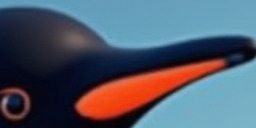
\includegraphics[width=78.500bp,height=39.250bp]{qual_tiles/nfe21_supp/033_seacache_crop.jpg}};
\node[anchor=north,inner sep=0] at (375.75,-163.55) {\num 34.36};
\node[anchor=north west,inner sep=0] at (416.50,-42.50) {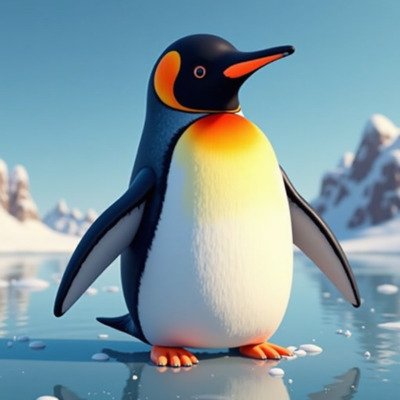
\includegraphics[width=78.500bp,height=78.500bp]{qual_tiles/nfe21_supp/033_ours_full.jpg}};
\draw[black,line width=1.3bp] (454.52,-48.63) rectangle (474.15,-58.45);
\draw[white,line width=0.6bp] (454.52,-48.63) rectangle (474.15,-58.45);
\node[anchor=north west,inner sep=0] at (416.50,-122.50) {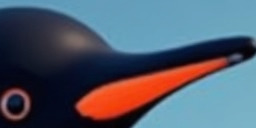
\includegraphics[width=78.500bp,height=39.250bp]{qual_tiles/nfe21_supp/033_ours_crop.jpg}};
\node[anchor=north,inner sep=0] at (455.75,-163.55) {\num \textbf{35.39}};
\node[anchor=south west,inner sep=0,text width=238.50bp,align=flush left,font=\prm] at (10.00,-208.95) {``An instqrumemnt used for cutting cloth, paper, axdz othr thdin mteroial, consamistng of two blades lad one on tvopb of the other and fhastned in tle mixdqdjle so as to bllow them txo be pened and closed by thumb and fitngesr inserted tgrough rings on kthe end oc thei vatndlzes.''};
\node[anchor=north west,inner sep=0] at (10.00,-210.95) {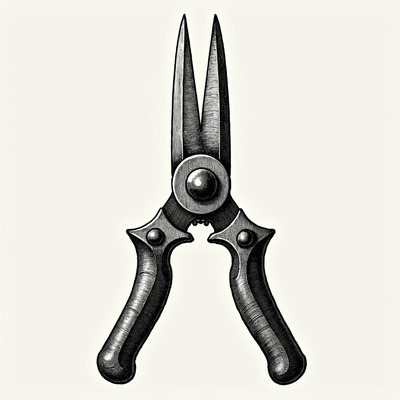
\includegraphics[width=78.500bp,height=78.500bp]{qual_tiles/nfe21_supp/111_reference_full.jpg}};
\draw[black,line width=1.3bp] (38.21,-248.97) rectangle (57.84,-258.79);
\draw[white,line width=0.6bp] (38.21,-248.97) rectangle (57.84,-258.79);
\node[anchor=north west,inner sep=0] at (10.00,-290.95) {
\includegraphics[width=78.500bp,height=39.250bp]{qual_tiles/nfe21_supp/111_reference_crop.jpg}};
\node[anchor=north,inner sep=0] at (49.25,-332.00) {\num\color{cInkTwo}PSNR (dB)};
\node[anchor=north west,inner sep=0] at (90.00,-210.95) {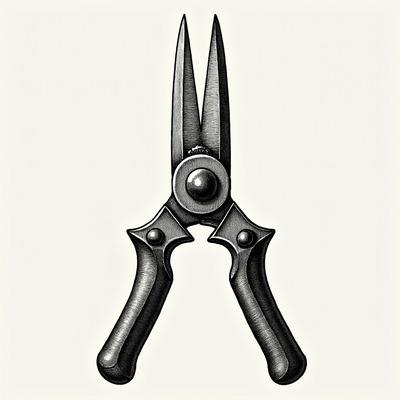
\includegraphics[width=78.500bp,height=78.500bp]{qual_tiles/nfe21_supp/111_seacache_full.jpg}};
\draw[black,line width=1.3bp] (118.21,-248.97) rectangle (137.84,-258.79);
\draw[white,line width=0.6bp] (118.21,-248.97) rectangle (137.84,-258.79);
\node[anchor=north west,inner sep=0] at (90.00,-290.95) {
\includegraphics[width=78.500bp,height=39.250bp]{qual_tiles/nfe21_supp/111_seacache_crop.jpg}};
\node[anchor=north,inner sep=0] at (129.25,-332.00) {\num 23.42};
\node[anchor=north west,inner sep=0] at (170.00,-210.95) {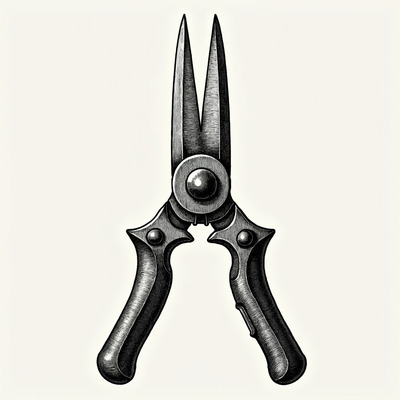
\includegraphics[width=78.500bp,height=78.500bp]{qual_tiles/nfe21_supp/111_ours_full.jpg}};
\draw[black,line width=1.3bp] (198.21,-248.97) rectangle (217.84,-258.79);
\draw[white,line width=0.6bp] (198.21,-248.97) rectangle (217.84,-258.79);
\node[anchor=north west,inner sep=0] at (170.00,-290.95) {
\includegraphics[width=78.500bp,height=39.250bp]{qual_tiles/nfe21_supp/111_ours_crop.jpg}};
\node[anchor=north,inner sep=0] at (209.25,-332.00) {\num \textbf{25.97}};
\node[rotate=90,anchor=south,inner sep=0] at (6.80,-270.57) {\sub Median gain};
\node[anchor=south west,inner sep=0,text width=238.50bp,align=flush left,font=\prm] at (256.50,-208.95) {``An IT-guy trying to fix hardware of a PC tower is being tangled by the PC cables like Laokoon. Marble, copy after Hellenistic original from ca. 200 BC. Found in the Baths of Trajan, 1506.''};
\node[anchor=north west,inner sep=0] at (256.50,-210.95) {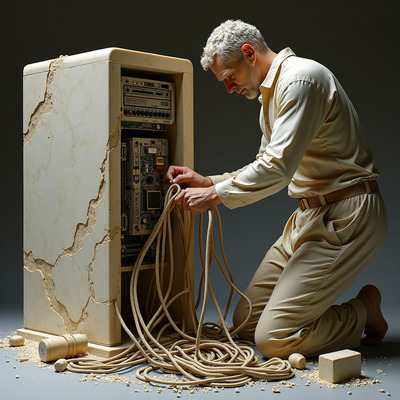
\includegraphics[width=78.500bp,height=78.500bp]{qual_tiles/nfe21_supp/152_reference_full.jpg}};
\draw[black,line width=1.3bp] (287.16,-242.23) rectangle (306.79,-252.04);
\draw[white,line width=0.6bp] (287.16,-242.23) rectangle (306.79,-252.04);
\node[anchor=north west,inner sep=0] at (256.50,-290.95) {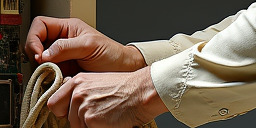
\includegraphics[width=78.500bp,height=39.250bp]{qual_tiles/nfe21_supp/152_reference_crop.jpg}};
\node[anchor=north,inner sep=0] at (295.75,-332.00) {\num\color{cInkTwo}PSNR (dB)};
\node[anchor=north west,inner sep=0] at (336.50,-210.95) {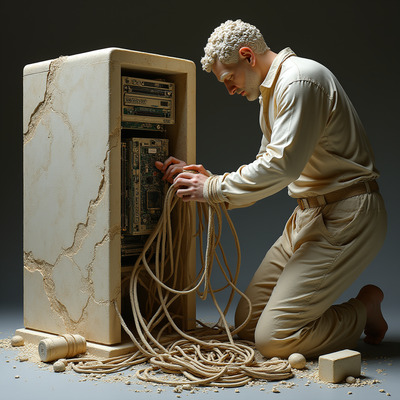
\includegraphics[width=78.500bp,height=78.500bp]{qual_tiles/nfe21_supp/152_seacache_full.jpg}};
\draw[black,line width=1.3bp] (367.16,-242.23) rectangle (386.79,-252.04);
\draw[white,line width=0.6bp] (367.16,-242.23) rectangle (386.79,-252.04);
\node[anchor=north west,inner sep=0] at (336.50,-290.95) {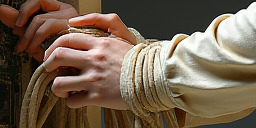
\includegraphics[width=78.500bp,height=39.250bp]{qual_tiles/nfe21_supp/152_seacache_crop.jpg}};
\node[anchor=north,inner sep=0] at (375.75,-332.00) {\num 21.34};
\node[anchor=north west,inner sep=0] at (416.50,-210.95) {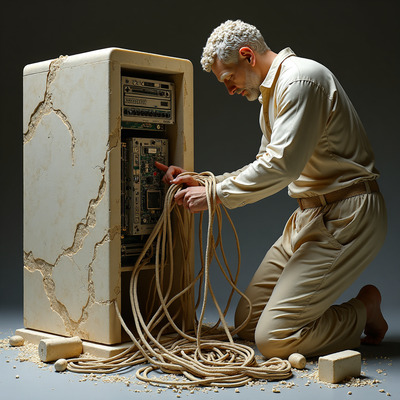
\includegraphics[width=78.500bp,height=78.500bp]{qual_tiles/nfe21_supp/152_ours_full.jpg}};
\draw[black,line width=1.3bp] (447.16,-242.23) rectangle (466.79,-252.04);
\draw[white,line width=0.6bp] (447.16,-242.23) rectangle (466.79,-252.04);
\node[anchor=north west,inner sep=0] at (416.50,-290.95) {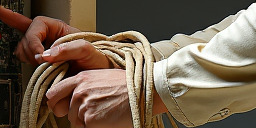
\includegraphics[width=78.500bp,height=39.250bp]{qual_tiles/nfe21_supp/152_ours_crop.jpg}};
\node[anchor=north,inner sep=0] at (455.75,-332.00) {\num \textbf{23.86}};
\node[anchor=south west,inner sep=0,text width=238.50bp,align=flush left,font=\prm] at (10.00,-361.20) {``A brown colored giraffe.''};
\node[anchor=north west,inner sep=0] at (10.00,-363.20) {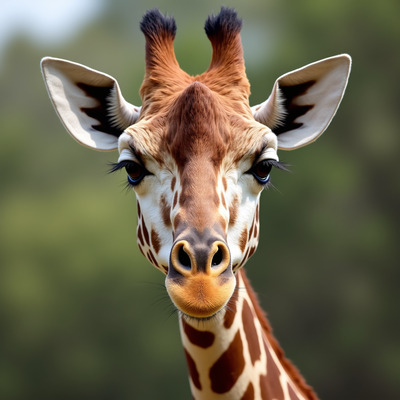
\includegraphics[width=78.500bp,height=78.500bp]{qual_tiles/nfe21_supp/014_reference_full.jpg}};
\draw[black,line width=1.3bp] (40.05,-414.72) rectangle (59.68,-424.53);
\draw[white,line width=0.6bp] (40.05,-414.72) rectangle (59.68,-424.53);
\node[anchor=north west,inner sep=0] at (10.00,-443.20) {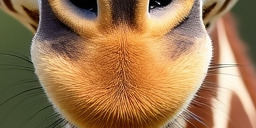
\includegraphics[width=78.500bp,height=39.250bp]{qual_tiles/nfe21_supp/014_reference_crop.jpg}};
\node[anchor=north,inner sep=0] at (49.25,-484.25) {\num\color{cInkTwo}PSNR (dB)};
\node[anchor=north west,inner sep=0] at (90.00,-363.20) {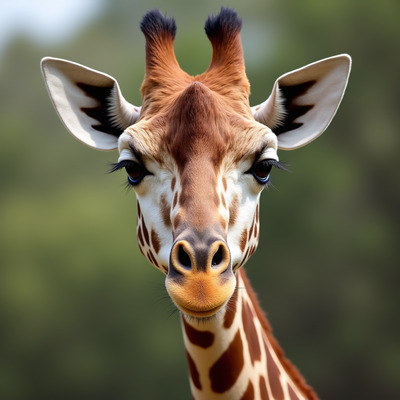
\includegraphics[width=78.500bp,height=78.500bp]{qual_tiles/nfe21_supp/014_seacache_full.jpg}};
\draw[black,line width=1.3bp] (120.05,-414.72) rectangle (139.68,-424.53);
\draw[white,line width=0.6bp] (120.05,-414.72) rectangle (139.68,-424.53);
\node[anchor=north west,inner sep=0] at (90.00,-443.20) {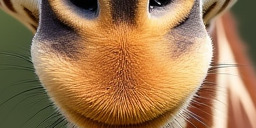
\includegraphics[width=78.500bp,height=39.250bp]{qual_tiles/nfe21_supp/014_seacache_crop.jpg}};
\node[anchor=north,inner sep=0] at (129.25,-484.25) {\num 32.38};
\node[anchor=north west,inner sep=0] at (170.00,-363.20) {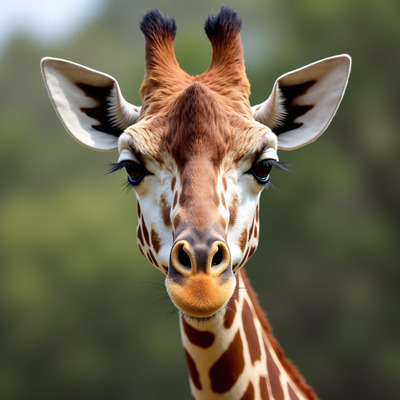
\includegraphics[width=78.500bp,height=78.500bp]{qual_tiles/nfe21_supp/014_ours_full.jpg}};
\draw[black,line width=1.3bp] (200.05,-414.72) rectangle (219.68,-424.53);
\draw[white,line width=0.6bp] (200.05,-414.72) rectangle (219.68,-424.53);
\node[anchor=north west,inner sep=0] at (170.00,-443.20) {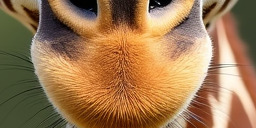
\includegraphics[width=78.500bp,height=39.250bp]{qual_tiles/nfe21_supp/014_ours_crop.jpg}};
\node[anchor=north,inner sep=0] at (209.25,-484.25) {\num \textbf{36.85}};
\node[rotate=90,anchor=south,inner sep=0] at (6.80,-422.82) {\sub Upper-quartile gain};
\node[anchor=south west,inner sep=0,text width=238.50bp,align=flush left,font=\prm] at (256.50,-361.20) {``A sphere made of kitchen tile. A sphere with the texture of kitchen tile.''};
\node[anchor=north west,inner sep=0] at (256.50,-363.20) {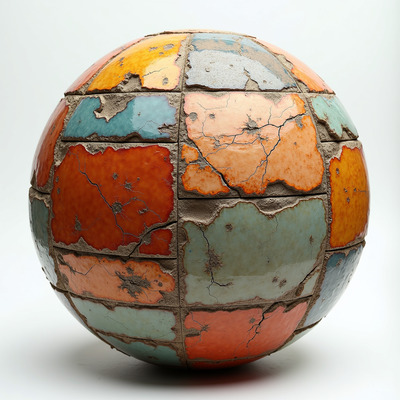
\includegraphics[width=78.500bp,height=78.500bp]{qual_tiles/nfe21_supp/058_reference_full.jpg}};
\draw[black,line width=1.3bp] (292.07,-372.40) rectangle (311.70,-382.21);
\draw[white,line width=0.6bp] (292.07,-372.40) rectangle (311.70,-382.21);
\node[anchor=north west,inner sep=0] at (256.50,-443.20) {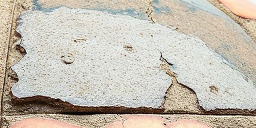
\includegraphics[width=78.500bp,height=39.250bp]{qual_tiles/nfe21_supp/058_reference_crop.jpg}};
\node[anchor=north,inner sep=0] at (295.75,-484.25) {\num\color{cInkTwo}PSNR (dB)};
\node[anchor=north west,inner sep=0] at (336.50,-363.20) {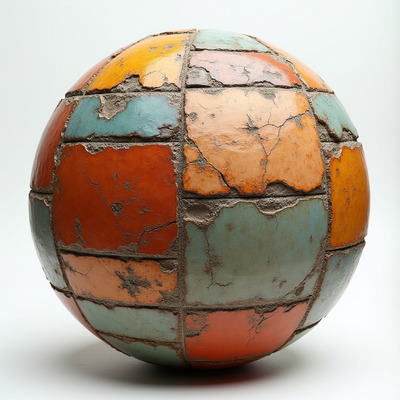
\includegraphics[width=78.500bp,height=78.500bp]{qual_tiles/nfe21_supp/058_seacache_full.jpg}};
\draw[black,line width=1.3bp] (372.07,-372.40) rectangle (391.70,-382.21);
\draw[white,line width=0.6bp] (372.07,-372.40) rectangle (391.70,-382.21);
\node[anchor=north west,inner sep=0] at (336.50,-443.20) {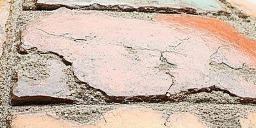
\includegraphics[width=78.500bp,height=39.250bp]{qual_tiles/nfe21_supp/058_seacache_crop.jpg}};
\node[anchor=north,inner sep=0] at (375.75,-484.25) {\num 22.40};
\node[anchor=north west,inner sep=0] at (416.50,-363.20) {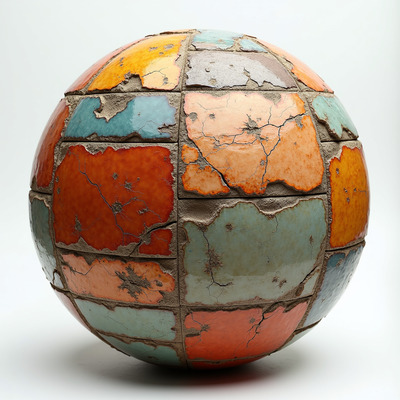
\includegraphics[width=78.500bp,height=78.500bp]{qual_tiles/nfe21_supp/058_ours_full.jpg}};
\draw[black,line width=1.3bp] (452.07,-372.40) rectangle (471.70,-382.21);
\draw[white,line width=0.6bp] (452.07,-372.40) rectangle (471.70,-382.21);
\node[anchor=north west,inner sep=0] at (416.50,-443.20) {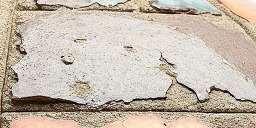
\includegraphics[width=78.500bp,height=39.250bp]{qual_tiles/nfe21_supp/058_ours_crop.jpg}};
\node[anchor=north,inner sep=0] at (455.75,-484.25) {\num \textbf{26.89}};
\end{tikzpicture}
\end{document}
